\section{Motivation}\label{sec:motivation}

In 1916, Albert Einstein developed a theory of gravitation known as general relativity \cite{einsteinGR}.
This is a generalisation of special relativity that refines Newton's law of universal gravitation and changes our understanding of gravity from being a force to being a warping of space.
Notably, it accounted for the precession in the orbit of Mercury about the Sun, and preceded the detection of both gravitational time dilation \cite{gravTimeDilateDetect} and gravitational waves \cite{gravWaveDetectPaper}, which it initially predicted.
At the centre of general relativity are the Einstein Field Equations \cite{einsteinFieldEquations},
\begin{equation}
G_{ab}+\Lambda g_{ab}=\frac{8\pi G}{c^4}T_{ab},
\end{equation}
where $\Lambda$ and $G$ are constants (cosmological and gravitational respectively), $G_{ab}$, $T_{ab}$, and $g_{ab}$ are tensors (Einstein, stress-energy, and metric respectively), and $c$ is the speed of light in a vacuum.
The Einstein tensor $G_{ab}$ is defined in terms of the Ricci tensor in the following equation \cite{einsteinFieldEquations},
\begin{equation}
G_{ab}=R_{ab}-\frac{1}{2}Rg_{ab},
\end{equation}
the definition of which can be found in Appendix \ref{apx:einsteintensor}.
When these equations are solved for exact solutions that are physically sensible, we produce metrics.
The Schwarzschild metric is an exact solution of significant importance, as it was the first one, which was discovered in 1916 by Karl Schwarzschild \cite{schwarz1916}.
This metric will be the first of two that will be used in this thesis; the other of which is the Kerr metric, which was discovered in 1963 by Roy Kerr \cite{kerrMetric}.

In general relativity, lines called geodesics are to curved spaces what straight lines are to flat spaces, so in curved spaces we understand geodesics to be ``locally straight lines".
More rigorously, we may define these geodesics by demanding the parallel transport of their tangent vectors \cite{schutzFirstGR}.
Given a metric we can define the Christoffel symbols\footnote{The semi-colon notation in the subscript of the metrics is to be understood as partial differentiation with respect to the variable after the semi-colon.} \cite{einsteinFieldEquations},
\begin{equation}\label{eqn:christoffel}
\Gamma^\alpha{}_{\beta\delta}=\frac{1}{2}g^{\alpha \gamma}(g_{\gamma\beta;\delta}+g_{\gamma\delta;\beta}-g_{\beta\delta;\gamma}),
\end{equation}
which are used to create the geodesic equations, which in turn give us information about the paths of orbiting test bodies.
As defined by Eqn.~(127) in \textit{The Mathematical Theory of Black Holes} by Chandrasekhar \cite{chandraBook}, the geodesic equations are
\begin{equation}\label{eqn:geodesic_eqn}
    \dv[2]{x^\alpha}{\lambda}+\Gamma^{\alpha}{}_{\beta\delta}\dv{x^\beta}{\lambda}\dv{x^\delta}{\lambda}=0.
\end{equation}

A current topic of interest in the research of general relativity that makes use of geodesy is gravitational wave detection -- specifically, the detection of gravitational waves from Extreme Mass Ratio Inspirals (EMRIs).
Noting the paper from Lukes-Gerakopoulos and Witzany \cite{emriExplained}, an EMRI consists of a two-body orbital problem where a stellar black hole orbits a supermassive black hole and the orbit of the smaller body, as a result of the radiation reaction force, eventually tends towards the event horizon of the larger black hole and crosses it.
The orbit of the smaller mass in an EMRI can be approximated to leading-order through geodesics, allowing for a more comprehensive understanding of the system as a whole.
Currently, the smallest observed mass of a stellar black hole is $3.3^{+2.8}_{-0.7}M_{\odot}$ \cite{smallStellar}, while the largest is $62^{+4}_{-4}M_{\odot}$, whereas the supermassive black hole at the centre of the Milky Way, Sgr A$^*$, has a mass of $4.154^{+0.014}_{-0.014}\times 10^6 M_{\odot}$ \cite{SgrAMass}; however, this is relatively small when considering other supermassive black holes.
For comparison, as of March 29th, 2023, a paper was published that stated the black hole at the centre of the galaxy Abell 1201 BCG has an approximate mass of $3.27^{+2.12}_{-2.12}\times 10^{10} M_{\odot}$ \cite{abellSMBH}, which is four orders of magnitude greater than the mass of Sgr A$^*$.

In an EMRI, each orbit of the smaller body about the bigger one emits gravitational waves, which researchers are endeavouring to detect.
The first successful detection was performed in 2015 by the Laser Interferometer Gravitational-wave Observatory (LIGO) detector of the National Science Foundation \cite{gravWaveDetectPaper}.
In Fig.~\eqref{fig:interferometerExample} we can see an example of the construction of this style of interferometer, where the goal is to facilitate multiple sources of laser light merging to create an interference pattern.
In the case of LIGO, it consists of two arms, each 4km in length, arranged in an ``L" shape; these arms are much longer than the original interferometers of the same type when they were first used in the 19th century, which had arms less than 2 metres in length.
The extra length possessed by the arms of the LIGO interferometer allow it to measure incredibly small interferences in the light path -- CalTech states that LIGO is capable of measurements as small as $1\times10^{-19}$ metres \cite{LIGOSummary}.
To better understand the magnitude of this distance, it is $1\times10^{-4}$ times the width of a proton; this is larger than the effective cross section of a high-energy neutrino but smaller than the classical electron radius.
Two more interferometers which are in use today are the Virgo interferometer by the European Gravitational Observatory and the Kamioka Gravitational Wave Detector (KAGRA) by the Institute for Cosmic Ray Research.
These three interferometers form the LIGO-Virgo-KAGRA (LVK) collaboration.
There is also a satellite interferometer being developed by the European Space Agency called LISA (Laser Interferometer Space Antenna) which is set to launch in 2037 \cite{LISASummary}.

\begin{figure}
    \centering
    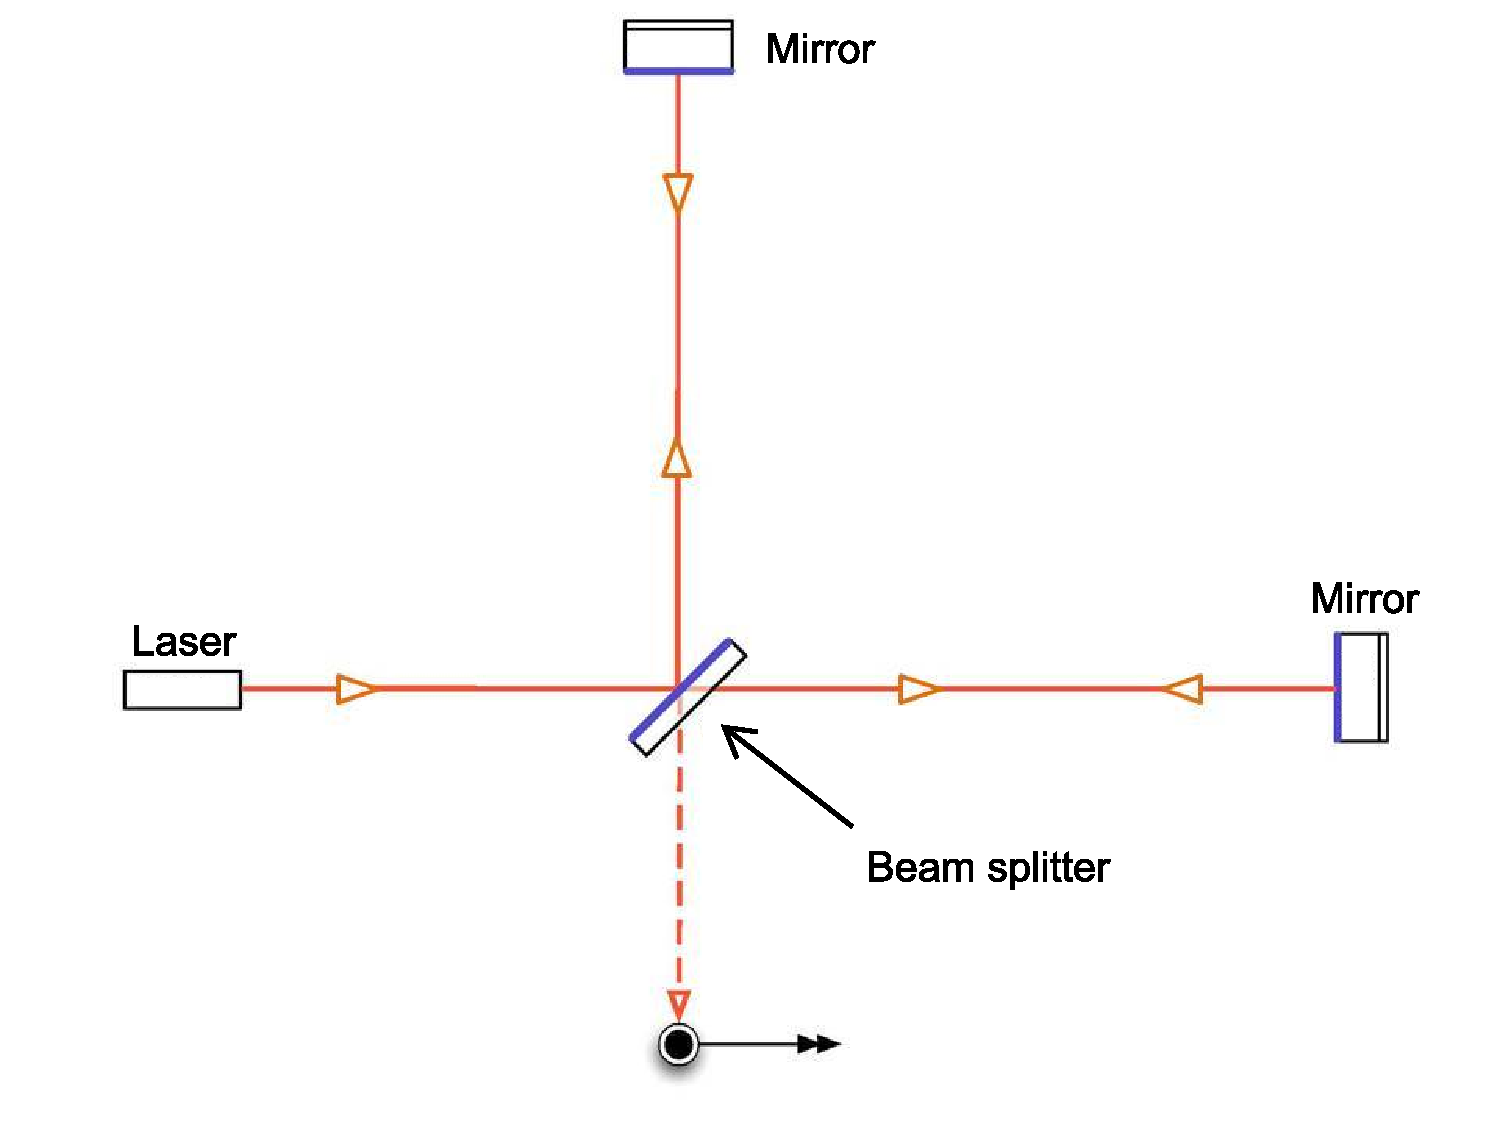
\includegraphics[width=0.55\textwidth]{images/Basic_michelson_labeled.pdf}
    \caption[Example of an interferometer]{An example of an interferometer. A laser is emitted and passes through a beam-splitter, which sends the laser down two different arms, each 4km long. These components of the laser beam will hit a mirror at the end of these arms and return, where they will make an interference pattern called ``fringes". At the very end, there is a photodetector that will measure these fringes and produce results. Credit: CalTech~\cite{LIGOSummary}.}
    \label{fig:interferometerExample}
\end{figure}

The study of geodesics and geodesic motion outside of general relativity has applications in a diverse range of disciplines.
In chemical physics, geodesic motion is used to understand molecular dynamics through computer simulations by examining the constant-potential-energy hypersurface of a system of particles \cite{chemPhysApp}.
In aeronautical engineering, a greater understanding of geodesics allowed for the cancellation of torsional load on a number of aircraft models, meaning less material was required to support the structure of the plane and offered more space within the centre for critical cargo \cite{aircraftApp}.
While in UV mapping (or surface remeshing), the computation of geodesics along surfaces allows for the embedding of a high-dimensional space in a low-dimensional space where Euclidean distances between points can be preserved to a reasonable degree.
This specific technique is how we can convert from a sphere, $\mathbb{S}^2\subset \mathbb{R}^3$ (like a globe), to a plane, $\mathbb{R}^2$ (a map) \cite{surfaceMeshApp, uvMapApp}.


Understanding many instances of orbital motion begins with geodesics, such as the previously mentioned EMRIs, all the way down to satellites orbiting smaller masses, and what should be an unsurprising revelation given the title of this paper, orbital motion about a black hole.


\section{Introduction}\label{sec:introduction}

The first exact solution to the Einstein Field Equations was found by Karl Schwarzschild in 1916 \cite{schwarz1916} and, with later work by Johannes Droste \cite{drosteSchwarz}, gave rise to the Schwarzschild metric, which in its later form was solved for in a simpler way than how Schwarzschild originally derived it.
This metric allows for the analysis of orbital motion about black holes that possess neither electric charge nor angular momentum, although the condition regarding angular momentum can be loosened to allow for the analysis of slowly rotating masses \cite{schwarzSlowRot}.
The Euler-Lagrange equations are used to solve for the constants of motion and derive a set of ordinary differential equations (ODEs) that later in this thesis are solved numerically
This constitutes the first method of solving for the equations of motion for the orbiting test body.
Different methods of solving for the equations of motion are utilised as a test on the results, in which case it can be confidently assumed that both methods have produced correct solutions, if they agree.
Solving the geodesic equations, as defined in Eqn.~\eqref{eqn:geodesic_eqn}, constitutes the second method of solving for the equations of motion and opens the door for the analysis of orbital motion in the Schwarzschild metric.

Without parameterisation, orbits are discussed and defined by two constants, namely the energy, $E$, and the angular momentum, $L$, through which it is difficult to establish a visual understanding of the properties of an orbit.
It would be of great benefit if a simpler understanding and extrapolation of these properties could be achieved.
Hence, two parameterisations are introduced to allow for a more tangible formulation of orbital properties such as orbital radius, eccentricity, and extreme orbital points.
First, the $p$-$e$ parameterisation introduces two new variables: $p$, the \textit{semi-latus rectum}, and $e$, the \textit{eccentricity} of the orbit \cite{cutlerEtAl}.
These will be formally defined later in such a way as to satisfy the maximum and minimum radial turning points.
Discussing orbits becomes much simpler with this parameterisation, as now it is possible to describe an orbit based on its ``size", $p$, and ``non-circularity", $e$, rather than through its energy and angular momentum.
Secondly, the Darwin parameterisation, which we will later see, introduces the parameter $\chi$, which takes values from $0$ to $2\pi$.
This parameter produces an even simpler understanding of orbital maxima, minima, and periodicity of orbit, and facilitates the numerical integration of a number of equations relating to the frequencies of orbit.
It does this by changing the path of integration in the integrals needed to calculate these frequencies from multi-valued to single-valued.


Extending the knowledge provided by the Schwarzschild metric, Roy Kerr discovered another exact solution to the Einstein Field Equations in 1963 \cite{kerrMetric}: the Kerr metric.
The complexity of our system may be increased to examine a wider range of black holes by removing the condition that the black hole in question must possess zero angular momentum, as the Kerr metric is concerned with \textit{rotating} black holes with no electric charge\footnote{Soon after the discovery of the Kerr metric came the Kerr-Newman metric, which removed the condition that the black hole must have no electric charge. \cite{kerrNewmanMetric}}.
A more robust understanding of orbital motion may now be developed due to the introduction of this property, along with the fact that orbits outside the equatorial plane are now examined.
These specific orbits are interesting in Kerr black holes due to periodic behaviour in the polar coordinate, and are not examined in the Schwarzschild case due to the simplification caused by spherical symmetry.
However, an issue arises with how the Kerr metric is defined -- the radial and polar equations are coupled, and so another parameterisation is introduced called \textit{Mino time} which decouples them.
Now the frequencies for Kerr orbits, which are defined as a number of integrals, are derived in Mino time.
Upon integration, we obtain a straightforward method for calculating the periods of orbit, and the exploration of resonant orbits begins.

This is not a heavily investigated topic, although there are a number of researchers who have spent time analysing this phenomenon (see, e.g., \cite{brinkResonance, brinkKerrResonance, ruangsriCensusReso, meentEMRIReso}).
Using an external library in Mathematica\footnote{The specific library is the Black Hole Perturbation Toolkit \cite{BHPToolkit}}, values for the periods of orbit may be calculated.
The library also provides a robust tool for finding resonant orbits given both of the orbital parameters $a$ and $x$, and one of either $p$ or $e$.
The parameters $p$ and $e$ are the same as before, while $a$ is the spin of the black hole, and $x$ is the angle from the equatorial plane, or inclination angle.
An analysis is made regarding the relationship of these parameters to each other in resonant orbits, and an approximately linear relationship is observed.
Noticing this, a method of estimation is formed for finding resonant $p$ values given values for $x$ and $e$ in the case where $a=0.9$.

Note that the work done in this thesis is carried out in the geometrised unit system, such that $G=c=1$, and we take $M=1$. We also retain the signature $(-+++)$ throughout.